\chapter{Máquinas Virtuais}

O termo máquina virtual~\cite{roland} foi descrito na década de 1960 utilizando um termo de sistema operacional: uma abstração de software que enxerga um sistema físico (máquina real). Com o passar dos anos, o termo englobou um grande número de abstrações – por exemplo, Java Virtual Machine – JVM que não virtualiza um sistema real.

Ao invés de ser uma real, isto é, um computador real feito de hardware e executando um sistema operacional específico, uma máquina virtual~\cite{jamhour} é um computador fictício criado por um programa de simulação. Sua memória, processador e outros recursos são virtualizados. A virtualização é a interposição do software (máquina virtual) em várias camadas do sistema. É uma forma de dividir os recursos de um computador em múltiplos ambientes de execução.

Os emuladores são máquinas virtuais que simulam computadores reais. São bastante conhecidos os emuladores de vídeo games antigos e os emuladores de microcomputadores, como o VMware, o Bochs e o VM VirtualBox (software livre da Oracle).

\section{Instrusão de Servidores em Máquinas Virtuais}

Existem várias ameaças que atingem a Web~\cite{kurose} nos dias atuais e aumentam cada vez mais com o passar do tempo. Com a necessidade de criação de novas funcionalidades em um ambiente em crescimento, projetistas podem não ter dado a devida atenção para a segurança e essa problemática permiti a invasão de diversos serviços hospedados em servidores~\cite{raitz}.
		
\begin{figure}
	\begin{center}
    	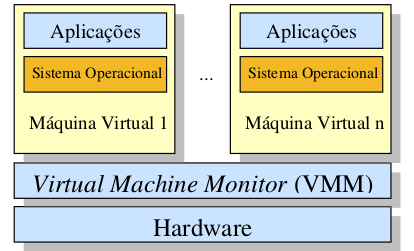
\includegraphics[width=0.7\textwidth]{RelacionamentoVMM}
    \end{center}
    \caption{Relacionamento das Máquinas Virtuais e do VMM~\cite{ferrazani}}
    \label{fig:RelacionamentoVMM}

\end{figure}
    
    
\section{Tipos de Máquinas Virtuais}
As máquinas virtuais podem ser divididas em três tipos:
\begin{itemize}
 \item   Tipo 1: Sistema em que o monitor é implementado entre o hardware e os sistemas convidados (guest system).
  \item  Tipo 2: Nele o monitor é implementado como um processo de um sistema operacional real, denominado sistema anfitrião (host system).
   \item Tipos Híbridos~\cite{nemeth}: Os monitores de tipo 1 e 2 raramente são usados em sua forma conceitual em implementações reais. Na prática, várias otimizações são inseridas nas arquiteturas apresentadas, com o objetivo principal de melhorar o desempenho das aplicações nos sistemas convidados. Como os pontos cruciais do desempenho dos sistemas de máquinas virtuais são as operações de E/S, as principais otimizações utilizadas em sistemas de produção dizem respeito a essas operações.
\end{itemize}
Outra importante categoria de máquinas virtuais são as máquinas virtuais para computadores fictícios projetados para uma finalidade específica. Atualmente a mais importante máquina virtual desta família é a JVM (máquina virtual Java). Existem simuladores para ela em quase todos os computadores atuais, desde computadores de grande porte até telefones celulares, o que torna as aplicações Java extremamente portáveis.

Uma importante vantagem sem duvida de se escrever código para uma máquina virtual é a de se poder compilar o código sem que seja perdida a portabilidade, melhorando-se a velocidade em relação à programação interpretada, que também é portátil, porém mais lenta, já que neste caso cada linha será traduzida e executada em tempo de execução, e no caso da máquina virtual cada mnemônico da máquina virtual é convertido no equivalente em linguagem de máquina (ou assembly) da máquina real.

\section{Vantagens}
\begin{itemize}
    \item Facilita o aperfeiçoamento e testes de novos sistemas operacionais.
    \item Possibilita a comparação de vários sistemas operacionais utilizando o mesmo equipamento.
    \item Executa diferentes sistemas operacionais sobre o mesmo hardware, simultaneamente.
    \item Simula alterações e falhas no hardware para testes ou reconfiguração de um sistema operacional, provendo confiabilidade e escalabilidade para as aplicações.
    \item Diminuição de custos com hardware.
    \item Facilidades no gerenciamento, migração e replicação~\cite{comer} de computadores, aplicações ou sistemas operacionais.
    \item Confiança e disponibilidade: A falha de um software não prejudica os demais serviços.
    \item Possibilidade do uso em Sistemas Distribuídos~\cite{dantas}.
    \item  Segurança: Usando máquinas virtuais, pode ser definido qual é o melhor ambiente para
executar cada serviço, com diferentes requerimentos de segurança, ferramentas diferentes e o sistema operacional mais adequado para cada serviço. Além disso, cada máquina virtual é isolada das demais. Usando uma máquina virtual para cada serviço, a
vulnerabilidade de um serviço não prejudica os demais.
\item  Confiança e disponibilidade: A falha de um software não prejudica os demais serviços.
\item Custo: A redução de custos é possível de ser alcançada com a consolidação de pequenos
servidores em outros mais poderosos. Essa redução pode variar de 29 a 64 porcento ~\cite{ferrazani}.
\item  Adaptação às diferentes cargas de trabalho: Variações na carga de trabalho podem ser
tratadas facilmente. Ferramentas autônomas podem realocar recursos de uma máquina virtual para a outra.
\item Balanceamento de carga: Toda a máquina virtual está encapsulada no VMM. Sendo assim é fácil trocar a máquina virtual de plataforma, a fim de aumentar o seu desempenho.
\item Suporte a aplicações legadas: Quando uma empresa decide migrar para um novo Sistema Operacional, é possível manter o sistema operacional antigo sendo executado em uma máquina virtual, o que reduz os custos com a migração. Vale ainda lembrar que
a virtualização pode ser útil para aplicações que são executadas em hardware legado~\cite{ferrazani}, que está sujeito a falhas e tem altos custos de manutenção. Com a virtualização desse hardware, é possível executar essas aplicações em hardwares mais novos, com custo de
manutenção mais baixo e maior confiabilidade.
 \end{itemize}
 
 
\section{Desvantagens}
\begin{itemize}
\item Segurança: As máquinas virtuais são menos seguras que as máquinas físicas pelo fato de existir o Virtual Machine Monitor. Este ponto é interessante, pois se o sistema operacional hospedeiro tiver alguma vulnerabilidade, todas as máquinas virtuais que estão hospedadas nessa máquina física estão vulneráveis, já que o VMM é uma camada de software, portanto,
como qualquer software, está sujeito a vulnerabilidades.
   \item Gerenciamento: Os ambientes virtuais necessitam ser, monitorados, configurados e salvos . Existem produtos que fornecem essas soluções, mas esse é o campo no qual estão os maiores investimentos na área de virtualização, justamente por se tratar de um dos maiores contratempos na implementação da virtualização.
    \item Desempenho: Atualmente, não existem métodos consolidados para medir o desempenho de ambientes virtualizados. No entanto, a introdução de uma camada extra de software entre o sistema operacional e o hardware, o VMM ou hypervisor, gera um custo de processamento superior ao que se teria sem a virtualização. Outro ponto importante de ressaltar é que não se sabe exatamente quantas máquinas virtuais podem ser executadas por processador, sem que haja o prejuízo da qualidade de serviço.
    \end{itemize}
 
 
\begin{figure}
	\begin{center}
    	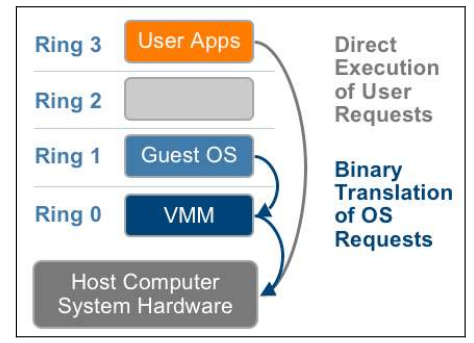
\includegraphics[width=0.7\textwidth]{virtualizacao}
    \end{center}
    \caption{Virtualização total em arquitetura x86~\cite{ferrazani}}
    \label{fig: virtualizacao}

\end{figure}
    
\section{Tipos de Virtualização}
Existem duas formas para implementação de Virtual Machine Monitor: Virtualização e Para-virtualização.

A virtualização total pode ser vista na Figura  \ref{fig: virtualizacao} tem por objetivo fornecer ao sistema operacional visitante uma réplica do hardware subjacente. Dessa forma, o sistema operacional visitante é executado sem modificações sobre o monitor de máquina virtual (VMM), o que traz alguns inconvenientes. O
primeiro é que o número de dispositivos a serem suportados pelo VMM é extremamente elevado.

Para resolver esse contratempo, as implementações da virtualização total usam dispositivos genéricos, que funcionam bem para a maioria dos dispositivos disponíveis, mas não garantem o usoda totalidade de sua capacidade. Outro inconveniente da virtualização total é o fato de o sistema operacional visitante não ter conhecimento de que está sendo executado sobre o VMM, então as instruções executadas pelo sistema operacional visitante devem ser testadas pelo VMM para que depois sejam executadas diretamente no hardware, ou executadas pelo VMM e simulada a execução para o sistema visitante. Por fim, o último inconveniente da virtualização total é o fato de ter que contornar alguns problemas gerados pela implementação dos sistemas operacionais, já que esses foram implementados para serem executados como instância única nas máquinas física, não disputando recursos com outros sistemas operacionais. Um exemplo desse último inconveniente é
uso de paginação na memória virtual, pois há a disputa de recursos entre diversas instâncias de sistemas operacionais, o que acarreta em uma queda do desempenho.
 

    


A para-virtualização é uma alternativa à virtualização total. Nesse modelo de virtualização, o sistema operacional é modificado para chamar o VMM sempre que executar uma instrução que possa alterar o estado do sistema, uma instrução sensível. Isso acaba com a necessidade de o VMM testar instrução por instrução, o que representa um ganho significativo de desempenho. Outro ponto
positivo da para-virtualização é que os dispositivos de hardware são acessados por drivers da própria máquina virtual, não necessitando mais do uso de drivers genéricos que inibiam o uso da capacidade total do dispositivo.

\begin{figure}
	\begin{center}
    	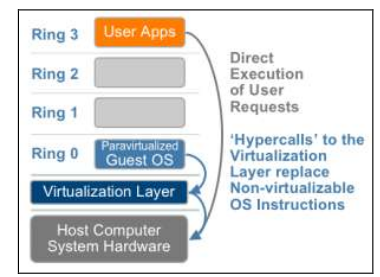
\includegraphics[width=0.7\textwidth]{virtualizacao2}
    \end{center}
    \caption{Para-virtualização em arquitetura x86~\cite{ferrazani}}
    \label{fig:virtualizacao2}

\end{figure}

Embora a para-virtualização apresentasse um ganho de desempenho significativo frente à virtualização total, essa disparidade tem sido superada devido à presença de instruções de virtualização nos processadores Intel e AMD, que favorecem a virtualização total. A tecnologia de virtualização da Intel é a IVT (Intel Virtualization Technology), codinome Vanderpool. A da AMD é a AMD-V (AMD-Virtualization), codinome Pacífica. Embora tenham sido desenvolvidas para o mesmo propósito, foram desenvolvidas de maneira independentes. Por esse motivo, há alguns problemas na portabilidade de máquinas virtuais de uma arquitetura Intel para a arquitetura AMD e vice-versa.

Portanto, tendo em vista as técnicas de virtualização, a decisão de qual melhor a técnica de virtualização para um dado ambiente está intimamente ligada a qual o processador da máquina física que vai hospedar as virtuais, bem como se o processador possui ou não uma extensão no seu conjunto de instruções que suporte a virtualização ~\cite{ferrazani}.

\section{Virtualização em segurança}
Alguns dos princípios básicos para garantir a segurança da informação:
\begin{itemize}
\item Confidencialidade: a informação somente está visível a sujeitos (usuários e/ou processos) explicitamente autorizados;
\item Disponibilidade: a informação deve estar prontamente disponível sempre que for necessária;
\item Integridade : a informação somente pode ser modificada por sujeitos explicitamente autorizados e de formas claramente definidas.
\end{itemize}
Outros critérios para garantir a segurança:
\begin{itemize}
\item Autenticidade: garante que a informação ou o usuário da mesma é autêntico, ou seja, garante que a entidade envolvida é quem afirma ser;
\item Não-repúdio : não é possível negar a existência ou autoria de uma operação que criou, modificou ou destruiu uma informação;
\item Auditoria: implica no registro das ações realizadas no sistema, identificando os sujeitos e recursos envolvidos, as operações realizadas, seus horários, locais e outros dados relevantes.
\end{itemize}

\section{Softwares para Virtualização}
\subsection{VMware}
VMware é um software/máquina virtual que permite a instalação e utilização de um sistema operacional dentro de outro dando suporte real a software de outros sistemas operativos.

Usando software de virtualização como o VMware é possível executar um ou mais sistemas operacionais simultaneamente num ambiente isolado, criando computadores completos (virtuais) a executar dentro de um computador físico que pode rodar um sistema operacional totalmente distinto. Do ponto de vista do utilizador e do software nem sequer se nota a diferença entre a máquina real e a virtual. É muito usado em centros de dados, pois permite criar redundância e segurança adicional sem recorrer a tantas máquinas físicas e distribuindo e aproveitando melhor os recursos das máquinas hospedeiras. Veja algumas aplicações do VMware:
\begin{itemize}
\item VMware Workstation
Utilizado no deskto e em ambientes de desenvolvimento. Atualmente está na versão 9.0.1, e roda em CPU's Intel e AMD de 32 e 64 bits. Permite rodar vários "computadores virtuais" dentro de um sistema operacional (Windows, versões GNU/LINUX, MAC OS, etc), cada um destes computadores pode rodar seu próprio sistema operacional. Possui alguns recursos importantes: Possibilidade de "unir" várias máquinas virtuais, permitindo que todas elas sejam iniciadas ou desligadas com um mesmo comando. Também é possível definir redes internas. Suporte a 3 modos de rede: Bridged (a máquina virtual é vista como um outro computador na rede, com IP obtido via DHCP); NAT (a máquina virtual se conecta ao computador host, que por sua vez se conecta à rede); e Host-Only (a máquina virtual apenas se conecta ao host).Possibilidade de criar registros instantâneos ("snapshots") de uma máquina virtual num dado momento. Assim, é possível testar configurações, e se elas derem errado pode-se reverter.
 \item VMware Server
 Dedicado ao uso em servidores de pequeno e médio porte. Tornou-se gratuito em 12 de Junho de 2006. É um produto de "entrada" para o mercado. Conta com boa parte dos recursos da versão Workstation, e adiciona recursos úteis ao seu uso em servidores, como o gerenciamento remoto (usando uma versão modificada do VNC). Isto resulta em perda de desempenho na interface gráfica, porém não é um problema para servidores que rodam "headless", ou seja, sem monitor ou interface gráfica.
\item VMware Player
Roda máquinas virtuais prontas; Oficialmente (Versões anteriores à versão 3.0), não é possível criar máquinas virtuais novas, mas é possível pular esta limitação de 3 formas: Instalando uma versão de avaliação do VMware Workstation e criando máquinas virtuais novas. Usando appliances (máquinas virtuais fornecidas pela comunidade, que operam como soluções prontas, onde basta apenas rodar). Usando sites não oficiais, como o EasyVMX. Usando a versão 3.0 ou superior.
\item VMware Fusion
Essa versão para o Mac OS X rodando em Macintosh com CPU Intel. O produto se encontra em sua quarta versão, com suporte inclusive a acereração 3d por hardware.
\end{itemize}


\subsection{VirtualBox}

VirtualBox é um software de virtualização desenvolvido pela empresa Innotek depois comprado pela Sun Microsystems que posteriormente foi comprada pela Oracle que, como o VMware Workstation, visa criar ambientes para instalação de sistemas distintos. Ele permite a instalação e utilização de um sistema operativo dentro de outro, assim como seus respectivos softwares, como dois ou mais computadores independentes, mas compartilhando fisicamente o mesmo hardware.

O VirtualBox tem um desenho extremamente modular com interfaces de programação interna bem definidas e um desenho cliente/servidor. Isso torna fácil o controle de várias interfaces de uma só vez. Por exemplo: você pode iniciar uma máquina virtual em uma máquina típica virtual ~\cite{stallings} de interface gráfica e, em seguida, controlar essa máquina a partir da uma linha de comando, ou possivelmente remotamente. O VirtualBox também vem com um kit completo desenvolvimento de software: embora seja de código aberto, você não tem que cortar a fonte de escrever uma nova interface para VirtualBox.

As definições de configuração de máquinas virtuais são armazenados em XML e são totalmente independentes das máquinas locais. Por isso, as definições podem ser facilmente transferidas para outros computadores.
O VirtualBox tem um software especial que pode ser instalado dentro das máquinas virtuais Windows e Linux para melhorar o desempenho e fazer integração muito mais perfeita. Entre os recursos fornecidos por essas adições clientes são integração do ponteiro do mouse o e soluções arbitrárias de tela.

Tal como muitos outras soluções de virtualização, para facilitar a troca de dados entre os hospedeiros e convidados, o VirtualBox permite a declaração dos diretórios de certos hospedeiros como "pastas compartilhadas", que pode ser acessadas de dentro de máquinas virtuais.


\subsection{\emph{Java Virtual Machine}}
Foi concebida para o desenvolvimento de pequenos aplicativos e
programas de controle de aparelhos eletrodomésticos e eletroeletrônicos, o Java mostrou-se ideal
para ser usada na rede internet. O que o torna tão atraente é o fato de programas escritos em Java
poderem ser executados virtualmente em qualquer plataforma, mas principalmente em Windows,
Unix e Mac.
Um programa fonte escrito em Java é traduzido pelo compilador para os bytecodes, isto é, o
código de máquina de um processador virtual, chamado Java Virtual Machine (JVM)~\cite{raitz} , que é o
monitor da máquina virtual Java.
A JVM é um programa capaz de interpretar os bytecodes produzidos pelo compilador. Com
isso, um programa Java pode ser executado em qualquer plataforma, desde que seja dotada de uma
JVM. É o caso dos programas navegadores mais populares, como o Netscape Navigator e o
Internet Explorer, que já vêm com uma JVM. A vantagem desta técnica é evidente: garantir uma
maior portabilidade para os programas Java em códigos-fonte e compilados.

\subsection{\emph{.NET Framework}}
O .Net, produto da Microsoft, também é uma máquina virtual, semelhante ao Java.
Desenvolvido sobre os padrões de Web Services XML, o .Net~\cite{raitz} possibilita que sistemas e
aplicativos, novos ou já existentes, conectem seus dados e transações, independente do sistema
operacional, tipo de computador ou de dispositivo móvel que sejam utilizados, ou de que
linguagem de programação tenha sido utilizada na sua criação.
A Common Language Infrastructure (CLI) contém a especificação dos seus principais
serviços. Ela implementa a tecnologia que permite que um aplicativo seja desenvolvido em
diversas linguagens de programação e executado num mesmo ambiente de execução. Ela é
suportada por diversos sistemas operacionais (sistemas Win32, FreeBSD, MAC OS X e em fase de
migração, o Linux), o que é de fundamental importância em aplicações distribuídas, como os
sistemas multiagentes.
Tudo isso é possível porque o Common Language Runtime (CLR) permite e fornece sistemas
de tipos comuns para todas as linguagens baseadas no .Net Framework.

\subsection{Microsoft Virtual PC}
O Microsoft Virtual PC 2004~\cite{raitz}, também conhecido como VirtualPC antes de ser adquirido da
Connectix pela Microsoft. Esta máquina virtual é muito parecida com o VMware. Pode ser
instalado e configurado na maioria dos sistemas operacionais baseados em Intel, sem a
necessidade de drivers específicos.
Algumas características são: suporte para até quatro adaptadores de rede por máquina;
configuração baseada na linguagem XML para facilitar a cópia da estação virtual; e suporte para
até 4 GB de memória.

\subsection{Xen}
O Xen~\cite{benevenuto} é um dos mais populares exemplos de para-virtualização. Na virtualização total, o sistema operacional visitante tenta executar tarefas protegidas e, por estarem no espaço de aplicação
do sistema operacional hospedeiro, não podem ser executadas. No entanto, o VMM intervem e
executa ou simula a execução dessas, o que reduz o desepenho da virtualização total. Já a para-
virtualização apresenta-se como uma alternativa a isso, na medida em que o sistema operacional
visitante é modificado para não tentar executar diretamente na CPU as tarefas protegidas~\cite{ferrazani}, mas
entregar essas ao VMM. Este tipo de virtualização tem um ganho de desempenho significativo
frente à total.
Uma das maiores vantagens do uso do Xen como VMM na para-virtualização é o fato de
que este apresenta um desempenho melhor do que os produtos de virtualização total, quando a
máquina física hospedeira não tem instruções de hardware de suporte a virtualização. No entanto,
há a necessidade de que o sistema visitante seja portado para o Xen, o que não chega a ser uma
desvantagem, já que os sistemas operacionais mais comuns no mercado têm versões para o Xen.
Alguns dos sistemas suportados pelo Xen são Linux, FreeBSD e Windows XP.
A tecnologia de virtualização provida pelo Xen difere da tecnologia do VMWare. O Xen
segue o conceito da para-virtualização, que fornece um conjunto de abstrações (processador virtual,
memória virtual, rede virtual etc.) sobre o qual diferentes sistemas podem ser portados~\cite{ferrazani}. As
abstrações não são necessariamente similares ao hardware da máquina física hospedeira.
Para entender como o Xen implementa a para-virtualização, é importante salientar dois
conceitos: o de domínio e o de hypervisor. Os domínios são as máquinas virtuais do Xen. Essas
podem ser de dois tipos, privilegiadas (domínio 0) e não-privilegiadas (domínio U). O hypervisor é
o responsável por controlar os recursos de comunicação, de memória e de processamento das
máquinas virtuais, mas não possui os drivers para manipular os dispositivos diretamente.
Quando a máquina hospedeira é iniciada, uma máquina virtual do domínio 0, privilegiado,
é criada. Esse domínio acessa uma interface de controle e executa aplicações de gerenciamento. As
máquinas virtuais dos domínios U só podem ser criadas, iniciadas e desligadas através do domínio
0. Na máquina virtual do domínio 0, é executado um Linux com núcleo modificado, que pode
acessar os recursos da máquina física, já que possui privilégios especiais, e ainda se comunicar com
as outras máquinas virtuais, domínio U.
O sistema operacional do domínio 0 tem que ser modificado para possuir os drivers de
dispositivo da máquina física e dois drivers que tratam requisições de acessos à rede e ao disco realizadas pelas máquinas virtuais do domínio U. Em suma, só a máquina virtual do domínio 0 tem
acesso direto aos recursos da máquina física, enquanto que as demais máquinas virtuais têm acesso
a uma abstração dos recursos, que para serem acessados, as máquina virtuais dos domínios U têm
que acessar através do domínio 0.

\begin{figure}
	\begin{center}
    	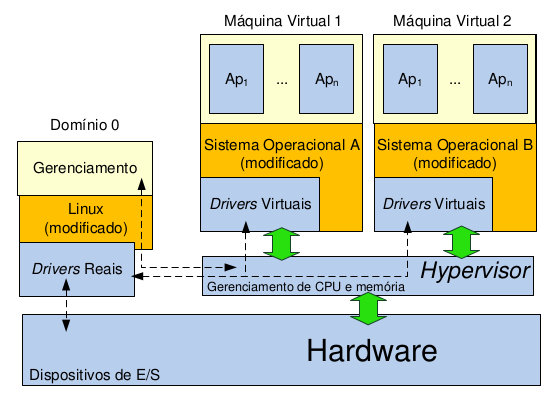
\includegraphics[width=0.7\textwidth]{ComponentesXen}
    \end{center}
    \caption{Componentes Xen~\cite{ferrazani}}
    \label{fig:ComponentesXen}

\end{figure}


Para a virtualização da memória, o Xen reserva para cada máquina virtual uma
determinada quantidade de memória, que pode ser alterada a qualquer momento sem a necessidade
de terminar ou reiniciar a máquina virtual. Cada máquina virtual pode ter uma ou mais interfaces de
rede virtuais. A comunicação entre as interfaces é implementada por dois token rings, um para
enviar e outro para receber.
Atualmente, o Xen conta também com um domínio no qual é feita a virtualização total, o
que permite que sistemas operacionais não modificados sejam executados sobre o hypervisor Xen.
Inicialmente, a escolha pela para-virtualização justificava-se pelo fato de que o ganho em
desempenho era muito maior do que com a virtualização total~\cite{ferrazani}. No entanto, com o advento das
arquiteturas AMD-V e Intel VT, arquitetura que dão o suporte de hardware para a virtualização, a
virtualização total passou a obter resultados de desempenho melhores que os da para-virtualização.
Vale ressaltar que o domínio de virtualização total disponível no Xen a partir da sua versão 3.0, só
pode ser usado nas máquinas hospedeiras que possuam suporte de hardware à virtualização.

